\documentclass{article}\usepackage[]{graphicx}\usepackage[]{color}
%% maxwidth is the original width if it is less than linewidth
%% otherwise use linewidth (to make sure the graphics do not exceed the margin)
\makeatletter
\def\maxwidth{ %
  \ifdim\Gin@nat@width>\linewidth
    \linewidth
  \else
    \Gin@nat@width
  \fi
}
\makeatother

\definecolor{fgcolor}{rgb}{0.345, 0.345, 0.345}
\newcommand{\hlnum}[1]{\textcolor[rgb]{0.686,0.059,0.569}{#1}}%
\newcommand{\hlstr}[1]{\textcolor[rgb]{0.192,0.494,0.8}{#1}}%
\newcommand{\hlcom}[1]{\textcolor[rgb]{0.678,0.584,0.686}{\textit{#1}}}%
\newcommand{\hlopt}[1]{\textcolor[rgb]{0,0,0}{#1}}%
\newcommand{\hlstd}[1]{\textcolor[rgb]{0.345,0.345,0.345}{#1}}%
\newcommand{\hlkwa}[1]{\textcolor[rgb]{0.161,0.373,0.58}{\textbf{#1}}}%
\newcommand{\hlkwb}[1]{\textcolor[rgb]{0.69,0.353,0.396}{#1}}%
\newcommand{\hlkwc}[1]{\textcolor[rgb]{0.333,0.667,0.333}{#1}}%
\newcommand{\hlkwd}[1]{\textcolor[rgb]{0.737,0.353,0.396}{\textbf{#1}}}%

\usepackage{framed}
\makeatletter
\newenvironment{kframe}{%
 \def\at@end@of@kframe{}%
 \ifinner\ifhmode%
  \def\at@end@of@kframe{\end{minipage}}%
  \begin{minipage}{\columnwidth}%
 \fi\fi%
 \def\FrameCommand##1{\hskip\@totalleftmargin \hskip-\fboxsep
 \colorbox{shadecolor}{##1}\hskip-\fboxsep
     % There is no \\@totalrightmargin, so:
     \hskip-\linewidth \hskip-\@totalleftmargin \hskip\columnwidth}%
 \MakeFramed {\advance\hsize-\width
   \@totalleftmargin\z@ \linewidth\hsize
   \@setminipage}}%
 {\par\unskip\endMakeFramed%
 \at@end@of@kframe}
\makeatother

\definecolor{shadecolor}{rgb}{.97, .97, .97}
\definecolor{messagecolor}{rgb}{0, 0, 0}
\definecolor{warningcolor}{rgb}{1, 0, 1}
\definecolor{errorcolor}{rgb}{1, 0, 0}
\newenvironment{knitrout}{}{} % an empty environment to be redefined in TeX

\usepackage{alltt}
%\usepackage{wrapfigure}
\usepackage{geometry}
\geometry{verbose,tmargin=2cm,bmargin=2cm,lmargin=2.5cm,rmargin=2.5cm}
\IfFileExists{upquote.sty}{\usepackage{upquote}}{}
\begin{document}





\title{Backcalculation of Undiagnosed HIV in WA State, 2005-2013}
\author{Martina Morris and Jeanette Birnbaum}
\maketitle

\section{Background}
This report uses the approach developed by Fellows et al\footnote{Fellows I, Morris M, Dombrowski J, Buskin S, Bennett A, and Golden M. \emph{A New HIV Testing History-Based Approach for Estimating the Undiagnosed Fraction of Persons with HIV Infection: Findings Suggest That Few HIV-Infected Men Who Have Sex with Men in King County, WA, U.S.A. Are  Undiagnosed.} Submitted, 2014.} to estimate HIV incidence and undiagnosed cases. The method combines data on the number of diagnoses per quarter with information on the distribution of the time between HIV infection and diagnosis, or TID. These two elements are used to ``backcalculate" the number of incident cases per quarter that must have occurred to result in the observed number of diagnoses. The number of undiagnosed cases per quarter are those cases who are estimated to have already been infected but not yet diagnosed in a given quarter.

Because TID is not directly observed, the method uses the time between last negative HIV test and diagnosis to approximate TID. The features of this approximation will define the uncertainty in the results.

\section{Data}
\subsection{Description of analytic sample}
Data from the advanced HIV/AIDS reporting system (eHARS) and the CDC treatment and testing history questionnaire (HIS) provided records for 25,233 HIV cases in WA state.\footnote{Provided by Jason Carr, Washington State Department of Health, June 13 2014}
\subsubsection{Exclusions}
Figure \ref{fig:exclusion} diagrams the construction of the analytic sample. We first restricted to cases diagnosed in WA state in the years 2005-2013. We further excluded cases diagnosed at age 16 or younger if their date of last negative test was missing, because the assumptions we use when date of last negative test is missing are not applicable to this age group (details given in Section~\ref{sec:methods}).

The final sample includes 4,744 cases.

% \begin{wrapfigure}{r}{0.5\textwidth}
%\begin{center}
%    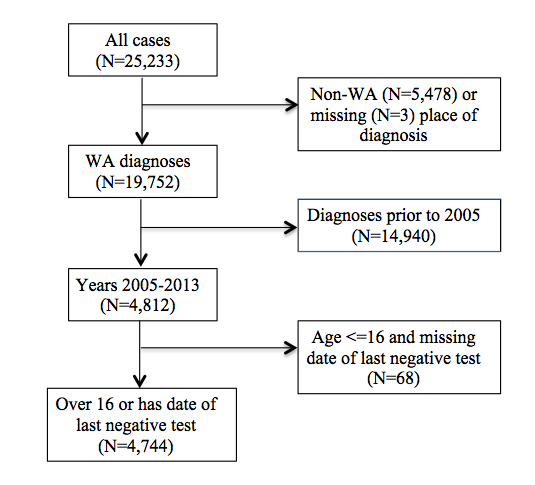
\includegraphics[width=0.48\textwidth]{exclusion_diagram}
%      \end{center}
%        \caption{A gull}
%    \end{wrapfigure}
    
\begin{figure}[!h]
  \centering
    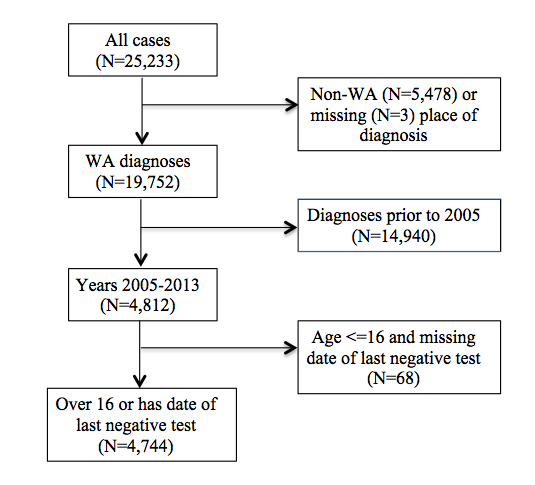
\includegraphics[width=3in]{exclusion_diagram}
    \caption{Construction of analytic sample}
    \label{fig:exclusion}
\end{figure}

\subsubsection{Sample characteristics}

Table \ref{tab:sample} describes the sample by age, race and mode of transmission. Column \% sums to 100\% within each characteristic. Six race/ethnicity groups are represented, White, Black, Hispanic, Asian, Native (NHoPI and AI/AN) and Multiracial, and three modes of transmission, MSM (including MSM/IDU), Hetero (including NIR and Female Presumed Hetero) and Blood/Needle (IDU, Ped, Hemo and Transfusion). 

For each level of these three characteristics, the table provides the breakdown of responses to the testing history question ``Have you ever had a prior negative HIV test?"  If a person ever had a negative test prior to diagnosis, they are in the \% Yes column. If they never had a negative test prior to diagnosis, they are in the \% No column. Those in the \% Missing column did not answer the question. These are row \%s that sum to 100\% across the \% Yes, \% No and \% Missing columns for each row. For example, 56\% of MSM have had a negative test, while 10\% have not. For 35\% of MSM, testing history is unknown. (These \%s sum to 101\% due to rounding error.) 

Table \ref{tab:sampleracebydx} further breaks down the sample into racial composition of cases within transmission modes. 


% latex table generated in R 3.0.3 by xtable 1.7-3 package
% Thu Jun 26 10:45:41 2014
\begin{table}[!h]
\centering
\caption{Composition of analytic sample by age, race and mode of transmission. Column \% sums to 100 within each characteristic. Availability of testing history data within each subgroup level is shown as row percents of \% Yes, \% No, and \% Missing)} 
\label{tab:sample}
{\small
\begin{tabular}{llrrrrr}
  \hline
Characteristic & Subgroup & N & Column \%  &  \% Yes &  \% No &  \% Missing \\ 
  \hline
Age Group & $\leq$20 & 168 & 4 & 49 & 18 & 33 \\ 
   & 21-25 & 655 & 14 & 54 & 12 & 34 \\ 
   & 26-30 & 664 & 14 & 52 & 10 & 38 \\ 
   & 31-35 & 738 & 16 & 49 & 10 & 41 \\ 
   & 36-40 & 706 & 15 & 41 & 11 & 48 \\ 
   & 41-45 & 627 & 13 & 43 & 12 & 46 \\ 
   & 46-50 & 515 & 11 & 35 & 12 & 52 \\ 
   & 51-55 & 310 & 7 & 35 & 16 & 48 \\ 
   & 56-60 & 203 & 4 & 37 & 23 & 40 \\ 
   & 61-65 & 101 & 2 & 23 & 21 & 56 \\ 
   & 66-70 & 44 & 1 & 34 & 18 & 48 \\ 
   & 71-85 & 13 & 0 & 46 & 15 & 38 \\ 
  Race/Ethnicity & White & 2773 & 58 & 50 & 10 & 40 \\ 
   & Black & 792 & 17 & 35 & 16 & 49 \\ 
   & Hisp & 732 & 15 & 39 & 13 & 48 \\ 
   & Asian & 220 & 5 & 30 & 23 & 47 \\ 
   & Native & 95 & 2 & 28 & 24 & 47 \\ 
   & Multi & 132 & 3 & 50 & 15 & 35 \\ 
  Mode of Transmission & MSM & 3135 & 66 & 56 & 10 & 35 \\ 
   & Hetero & 1334 & 28 & 22 & 18 & 60 \\ 
   & Blood/Needle & 275 & 6 & 29 & 16 & 55 \\ 
   \hline
\end{tabular}
}
\end{table}
% latex table generated in R 3.0.3 by xtable 1.7-3 package
% Thu Jun 26 10:45:41 2014
\begin{table}[!h]
\centering
\caption{Composition of racial groups within modes of transmission. Column \% sums to 100 within each mode. Availability of testing history data by mode-race subgroup levels is shown as row percents of \% Yes, \% No, and \% Missing} 
\label{tab:sampleracebydx}
{\small
\begin{tabular}{llrrrrr}
  \hline
Mode of Transmission & Race/Ethnicity & N & Column  \%  &  \%  Yes &  \%  No &  \%  Missing \\ 
  \hline
MSM & White & 2141 & 45 & 57 & 8 & 35 \\ 
  MSM & Black & 281 & 6 & 55 & 12 & 33 \\ 
  MSM & Hisp & 461 & 10 & 54 & 11 & 35 \\ 
  MSM & Asian & 112 & 2 & 49 & 13 & 38 \\ 
  MSM & Native & 45 & 1 & 44 & 22 & 33 \\ 
  MSM & Multi & 95 & 2 & 58 & 16 & 26 \\ 
  Hetero & White & 454 & 10 & 27 & 15 & 58 \\ 
  Hetero & Black & 476 & 10 & 25 & 17 & 58 \\ 
  Hetero & Hisp & 236 & 5 & 12 & 18 & 70 \\ 
  Hetero & Asian & 102 & 2 & 12 & 32 & 56 \\ 
  Hetero & Native & 39 & 1 & 10 & 31 & 59 \\ 
  Hetero & Multi & 27 & 1 & 26 & 15 & 59 \\ 
  Blood/Needle & White & 178 & 4 & 30 & 16 & 54 \\ 
  Blood/Needle & Black & 35 & 1 & 29 & 20 & 51 \\ 
  Blood/Needle & Hisp & 35 & 1 & 23 & 17 & 60 \\ 
  Blood/Needle & Asian & 6 & 0 & 0 & 33 & 67 \\ 
  Blood/Needle & Native & 11 & 0 & 27 & 9 & 64 \\ 
  Blood/Needle & Multi & 10 & 0 & 40 & 10 & 50 \\ 
   \hline
\end{tabular}
}
\end{table}


Minor assumptions made during data cleaning are given in Section~\ref{sec:missdata}.

\label{sec:sample}
\subsection{Time trends in diagnoses and testing history}


\begin{knitrout}\footnotesize
\definecolor{shadecolor}{rgb}{0.969, 0.969, 0.969}\color{fgcolor}\begin{figure}[!h]


{\centering 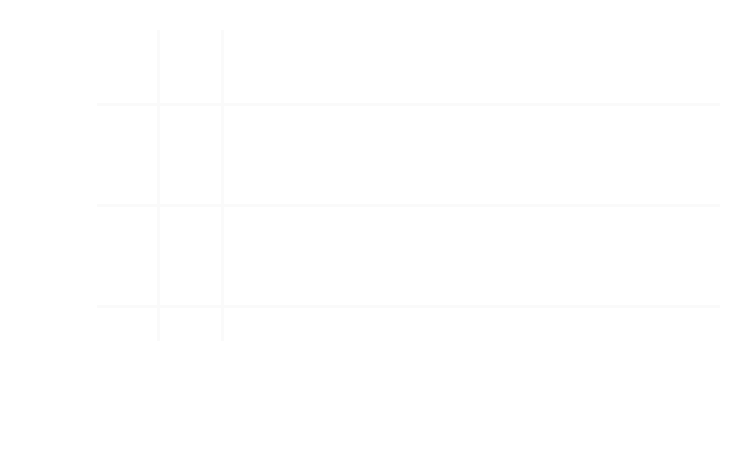
\includegraphics[width=\maxwidth]{figure/minimal-plot_diagnoses} 

}

\caption[Quarterly diagnosis counts over time]{Quarterly diagnosis counts over time\label{fig:plot_diagnoses}}
\end{figure}


\end{knitrout}



\begin{knitrout}\footnotesize
\definecolor{shadecolor}{rgb}{0.969, 0.969, 0.969}\color{fgcolor}\begin{figure}[!h]


{\centering 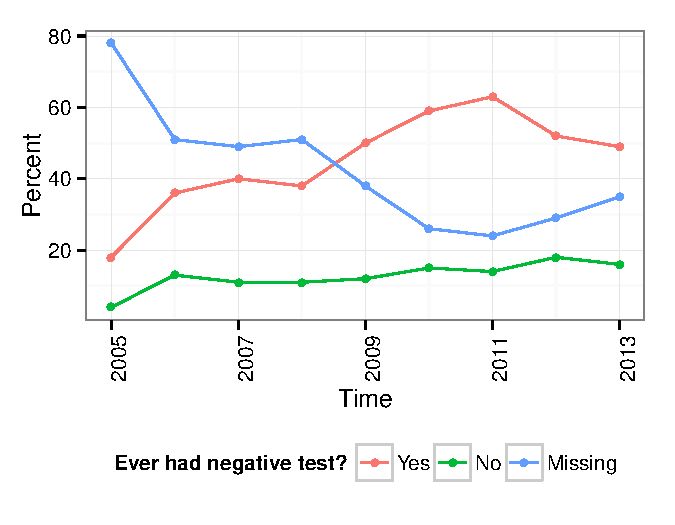
\includegraphics[width=\maxwidth]{figure/minimal-plot_time} 

}

\caption[Testing history responses over time (y-axis is in \%)]{Testing history responses over time (y-axis is in \%)\label{fig:plot_time}}
\end{figure}


\end{knitrout}

Figure \ref{fig:plot_diagnoses} shows a downward trend in quarterly diagnosis counts over time, and Figure \ref{fig:plot_time} shows the overall trend in testing history responses over time. The percent of missing responses appears to have increased in recent years.

Time rends by race and mode of diagnosis subgroups are given in Section~\ref{sec:testingBySubgroup}.

\section{Scenarios}
\label{sec:methods}

We consider three alternative scenarios to approximate the TID from the testing history data. The essential differences are described below, with more details in Section~\ref{sec:imputemiss}.

\begin{enumerate}
    \item \textbf{Base Case}  Missing testing history data are considered missing at random and are excluded from calculating the TID. The probability of infection is uniformly distributed between the time of last negative test and time of diagnosis.
    \item \textbf{Worst Case (Obs)} Missing testing history data are considered missing at random and are excluded from calculating the TID. Infection is assumed to occur immediately following the date of last negative test, a worst case assumption.
    \item \textbf{Worst Case (Miss)} Missing testing history data are imputed using the assumption that infection occurred either 18 years prior to diagnosis or at age 16, whichever is more recent. For cases with testing history, infection is assumed to occur immediately following the date of last negative test.
\end{enumerate}

In all three scenarios, cases who reported ``No" to ever having a negative test are also assumed to have a last negative test either 18 years prior to diagnosis or at age 16, whichever is more recent (see Section~\ref{sec:imputemiss} for more details). 
\section{Results}

\subsection{Time from infection to diagnosis (TID)}

Figure \ref{fig:plot_newfig1} shows the estimated distribution of TID in the analytic sample for each of the three scenarios. When worst case assumptions are made, the proportion of undiagnosed cases at shorter times since infection increases. The artifical drop at 18 years is a result of the assumption that all cases are diagnosed within 18 years.


\begin{knitrout}\footnotesize
\definecolor{shadecolor}{rgb}{0.969, 0.969, 0.969}\color{fgcolor}\begin{figure}[!h]


{\centering 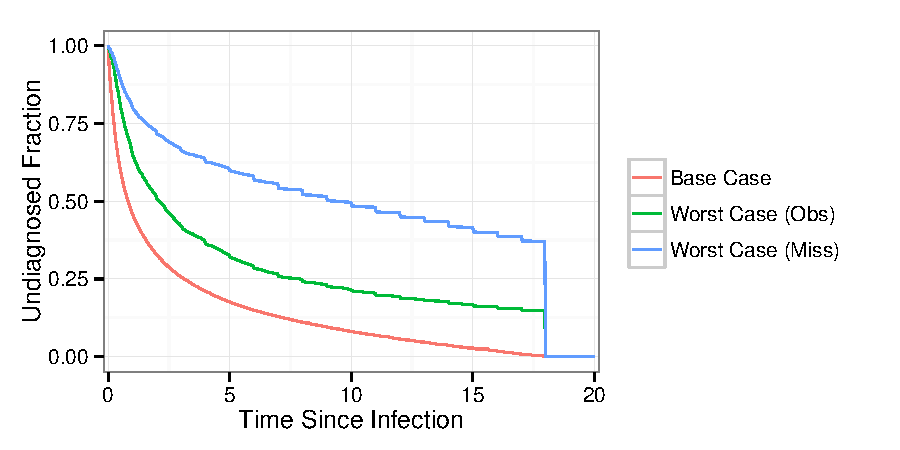
\includegraphics[width=\maxwidth]{figure/minimal-plot_newfig1} 

}

\caption[Time from infection to diagnosis (TID) under the three scenarios]{Time from infection to diagnosis (TID) under the three scenarios\label{fig:plot_newfig1}}
\end{figure}


\end{knitrout}

Times from infection to diagnosis by race and mode of diagnosis subgroups are given in Section~\ref{sec:TIDBySubgroup}.

\subsection{Incidence and undiagnosed cases}

We use observed quarterly diagnoses with each the three TID scenarios shown in Figure \ref{fig:plot_newfig1} to perform the backcalculation for each scenario. The estimated incidence and undiagnosed counts for each scenario are shown as quarterly counts in Figure \ref{fig:results_plot} and summarized over all quarters in Table \ref{tab:res_main}.



\begin{knitrout}\footnotesize
\definecolor{shadecolor}{rgb}{0.969, 0.969, 0.969}\color{fgcolor}\begin{figure}[!h]


{\centering 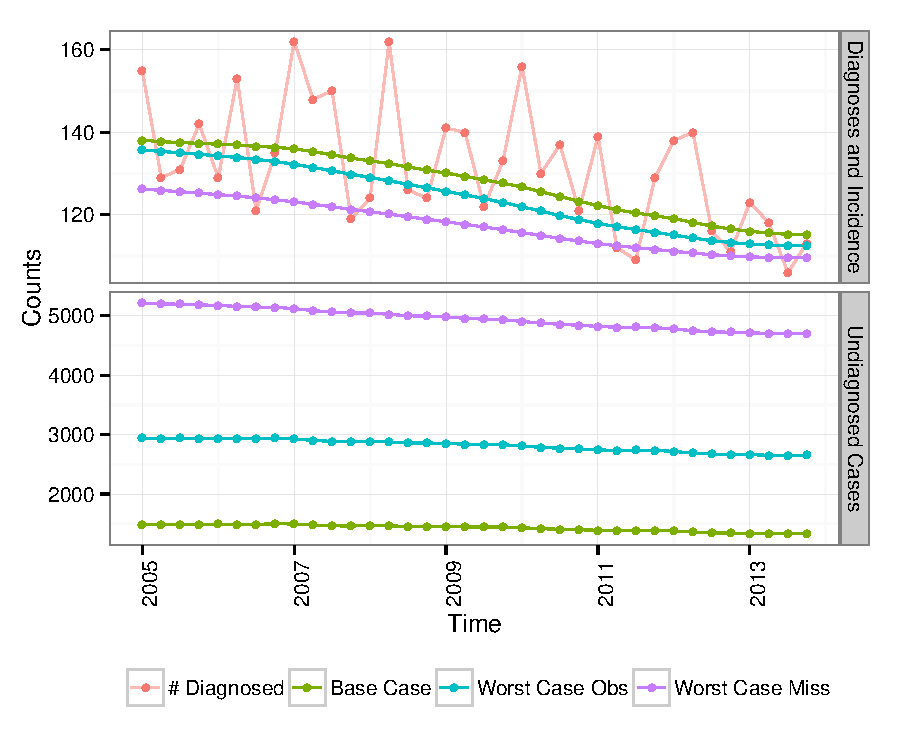
\includegraphics[width=\maxwidth]{figure/minimal-results_plot} 

}

\caption[Observed diagnoses and estimated quarterly and undiagnosed counts over 2005-2013 in WA state]{Observed diagnoses and estimated quarterly and undiagnosed counts over 2005-2013 in WA state\label{fig:results_plot}}
\end{figure}


\end{knitrout}


% latex table generated in R 3.0.3 by xtable 1.7-3 package
% Thu Jun 26 10:45:47 2014
\begin{table}[ht]
\centering
\caption{Observed diagnoses and estimated quarterly incidence and undiagnosed counts over 2005-2013 in WA state} 
\label{tab:res_main}
{\small
\begin{tabular}{lrrrrrr}
  \hline
 & Min  & 1st Qu  & Median & Mean & 3rd Qu  & Max  \\ 
  \hline
\# Diagnosed & 106 & 121 & 130 & 132 & 140 & 162 \\ 
  Incidence (Base Case) & 115 & 120 & 129 & 128 & 136 & 138 \\ 
  Incidence (Worst Case Obs) & 112 & 116 & 124 & 124 & 132 & 136 \\ 
  Incidence (Worst Case Miss) & 110 & 112 & 117 & 117 & 123 & 126 \\ 
  Undiagnosed (Base Case) & 1329 & 1386 & 1446 & 1429 & 1480 & 1501 \\ 
  Undiagnosed (Worst Case Obs) & 2652 & 2735 & 2836 & 2816 & 2910 & 2942 \\ 
  Undiagnosed (Worst Case Miss) & 4700 & 4807 & 4952 & 4950 & 5098 & 5217 \\ 
   \hline
\end{tabular}
}
\end{table}




Estimated incidence and undiagnosed counts by race and mode of diagnosis subgroups are given in Section~\ref{sec:undiagBySubgroup}.

\appendix
\section{Assumptions}
\subsection{Assumptions for missing or inconsistent data}
\label{sec:missdata}
The following assumptions were made during data cleaning:
\begin{table}[h]
\centering
\caption{Assumptions for missing or inconsistent data}
\begin{tabular}{|p{8cm}|p{4cm}|c|}
  \hline
Issue & Assumption & Cases Affected \\
  \hline
Year of diagnosis is recorded but quarter is not & Quarter is randomly assigned & 9 \\
  \hline
Case responded ``No'' or missing to ``Ever had negative test?" but has a date of last negative test & Change response to ``Yes" & 17 \\
\hline
Case responded ``Yes'' to ``Ever had negative test?" but has no date of last negative test & Change response to ``No" & 83 \\
\hline
\end{tabular}
\label{tab:data_assumptions}
\end{table}

Note: the analysis assumes that that there are a negligible number of cases whose HIV/AIDS diagnosis is never captured by eHARS.

\subsection{Assumptions for TID}
\label{sec:imputemiss}

As described in Section~\ref{sec:methods}, we construct three scenarios for TID that use different assumptions for missing data and the precise time of infection within the window between last negative test and diagnosis. 

\paragraph{Missing data} There are two ways we can treat cases whose date of last negative test is not known. The first is to exclude them when TID is computed, which assumes that their data are missing at random. This is reasonable only if the cases who do have a date of last negative test are representative of those who do not. Alternatively, we can impute their date of last negative test using a worst case assumption, that the last negative test occurred either 18 years ago or at age 16, whichever is more recent. This assumption is based on data suggesting that 95\% of HIV infections will develop AIDS within 18 years\footnote{Liu, K.J, et al., \emph{A model-based approach for estimating the mean incubation period of transfusion-associated acquired-immunodeficiency-syndrome.} PNAS, 1986. 83(10):p.3051-3055.} and on the median age of sexual debut in the U.S. 

\paragraph{Time of infection within the window between negative test and diagnosis} There are also two ways we can assign the precise time of infection within the possible infection window. The first is to assume that infections are uniformly distributed within the window, i.e. there is equal probability of infection at each time point within the window. The second is a worst case assumption, that infection occurred immediately after the negative test.

\paragraph{Assumptions for all scenarios} We additionally make three assumptions in all three scenarios. The first is that those who repond ``No" to the question ``Ever had a negative test?" have a date of last negative test imputed using the minimum of 18 years and age-16 approach described above. Since these cases confirmed never having a negative test, we use a worst case testing history to bound their infection window. The second is that dates of last negative test occurring more than 18 years prior to diagnosis are re-set to 18 years prior to diagnosis, to reflect a more likely maximum window in which infection could occur. Finally, we assume that the TID distrition does not change over time. In order to have enough cases to stably estimate the TID, we pool testing history data over all years. The time trends in the results are thus driven by the time trends in diagnosis counts.

\paragraph{} Table \ref{tab:TID_case_assumptions} outlines which assumptions are used for each of the three scenarios. Note that these assumptions influence the analysis solely through the TID distribution (see Figures \ref{fig:plot_newfig1}, \ref{fig:plot_modeTID} and \ref{fig:plot_raceTID}).

\begin{table}[!h]
\centering
\caption{Assumptions for each of the three cases used to approximate TID from testing history data}
\begin{tabular}{|p{7cm}|p{1.5cm}|p{1.5cm}|p{1.5cm}|p{1.5cm}|}
  \hline
Assumption & Base Case & Worst Case (Obs) & Worst Case (Miss) & Cases Affected \\ 
  \hline
Data are missing at random & X & X &  & 2104 \\
  \hline
Those with missing testing history are given a TID that is the minimum of 18 years or their age at diagnosis minus 16 years &  &  & X & 2104 \\
   \hline
Time of infection is uniformly distributed across the TID period  & X &  &   & All \\
  \hline
Infection occurs immediately after last negative test &  & X & X & All \\
  \hline
Those who never had a negative test are given a TID that is the minimum of 18 years or their age at diagnosis minus 16 years & X & X & X & 592 \\
  \hline
TID is capped at 18 years & X & X & X & 20 \\
  \hline
TID is stationary over time & X & X & X & All \\
  \hline
\end{tabular}
\label{tab:TID_case_assumptions}
\end{table}


\section{Subanalyses by Race and Mode of Diagnosis}
\subsection{Trends in diagnoses and testing history}
\label{sec:testingBySubgroup}

Figure \ref{fig:plot_diagnoses_subgroup} shows the trend in quarterly diagnoses for subgroups over time.  Figure \ref{fig:plot_modetime} shows the yearly trend in testing history by mode of transmission, and Figure \ref{fig:plot_racetime} shows the trend by race. Trends appear similar across subgroups, with variations in the levels of yes, no and missing responses each year.

\begin{knitrout}\footnotesize
\definecolor{shadecolor}{rgb}{0.969, 0.969, 0.969}\color{fgcolor}\begin{figure}[!h]


{\centering 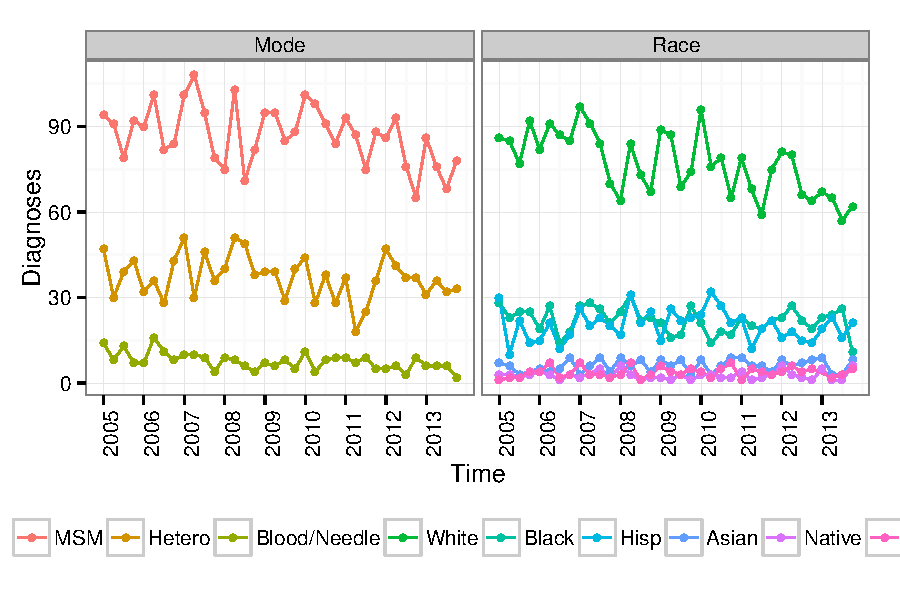
\includegraphics[width=\maxwidth]{figure/minimal-plot_diagnoses_subgroup} 

}

\caption[Quarterly diagnosis counts over time, by mode of transmission and race]{Quarterly diagnosis counts over time, by mode of transmission and race\label{fig:plot_diagnoses_subgroup}}
\end{figure}


\end{knitrout}

\begin{knitrout}\footnotesize
\definecolor{shadecolor}{rgb}{0.969, 0.969, 0.969}\color{fgcolor}\begin{figure}[!h]


{\centering 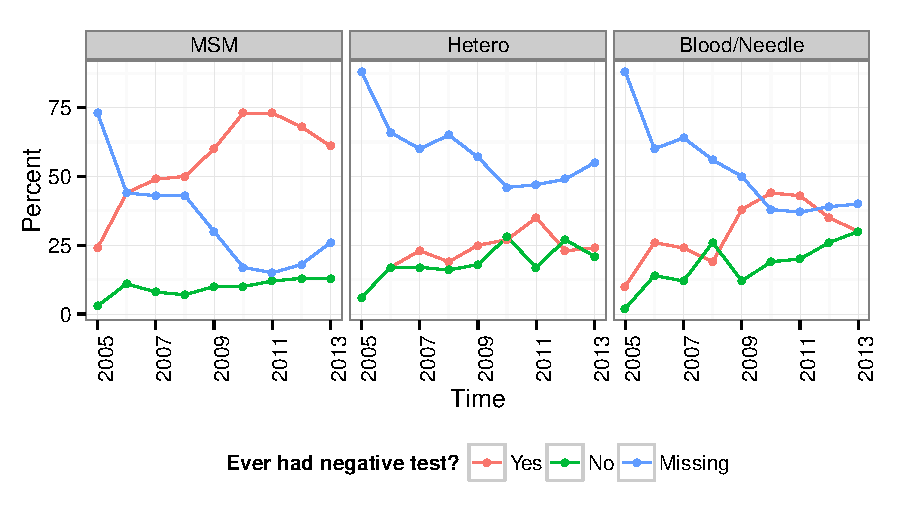
\includegraphics[width=\maxwidth]{figure/minimal-plot_modetime} 

}

\caption[Testing history responses over time, by mode of transmission (y-axis is in \%)]{Testing history responses over time, by mode of transmission (y-axis is in \%)\label{fig:plot_modetime}}
\end{figure}


\end{knitrout}


\begin{knitrout}\footnotesize
\definecolor{shadecolor}{rgb}{0.969, 0.969, 0.969}\color{fgcolor}\begin{figure}[hb]


{\centering 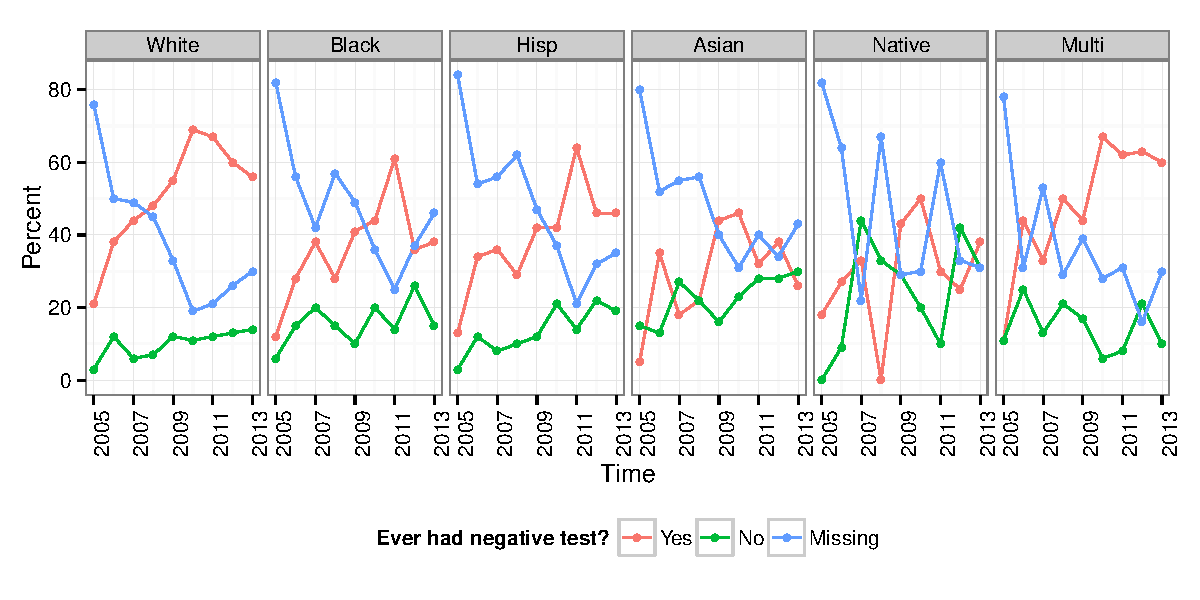
\includegraphics[width=\maxwidth]{figure/minimal-plot_racetime} 

}

\caption[Testing history responses over time, by race (y-axis is in \%)]{Testing history responses over time, by race (y-axis is in \%)\label{fig:plot_racetime}}
\end{figure}


\end{knitrout}


\subsection{Times from infection to diagnosis}
\label{sec:TIDBySubgroup}
The estimated TIDs for each of the three scenarios is shown by mode of transmission in Figure \ref{fig:plot_modeTID} and by race in Figure \ref{fig:plot_raceTID}.

\begin{knitrout}\footnotesize
\definecolor{shadecolor}{rgb}{0.969, 0.969, 0.969}\color{fgcolor}\begin{figure}[hb]


{\centering 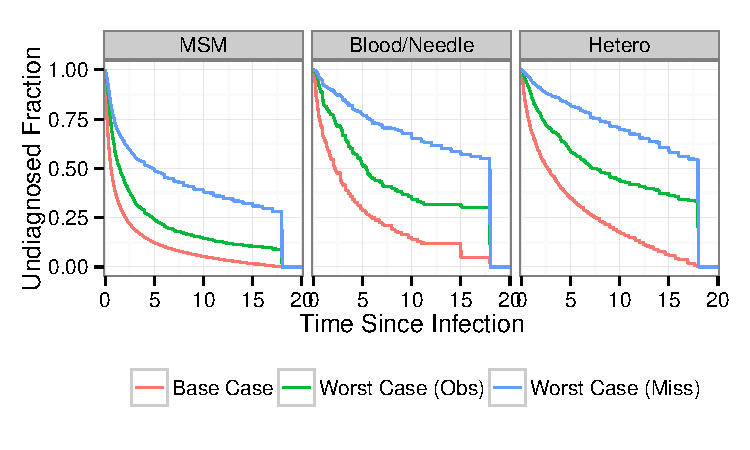
\includegraphics[width=\maxwidth]{figure/minimal-plot_modeTID} 

}

\caption[Time from infection to diagnosis (TID) under the three scenarios, by mode]{Time from infection to diagnosis (TID) under the three scenarios, by mode\label{fig:plot_modeTID}}
\end{figure}


\end{knitrout}


\begin{knitrout}\footnotesize
\definecolor{shadecolor}{rgb}{0.969, 0.969, 0.969}\color{fgcolor}\begin{figure}[hb]


{\centering 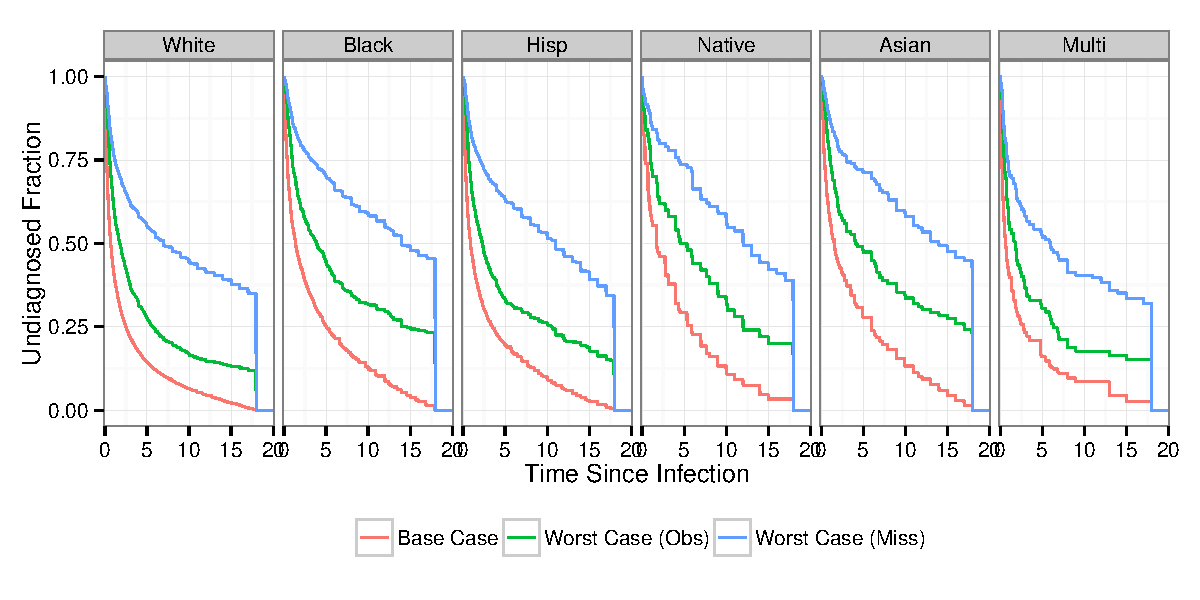
\includegraphics[width=\maxwidth]{figure/minimal-plot_raceTID} 

}

\caption[Time from infection to diagnosis (TID) under the three scenarios, by race]{Time from infection to diagnosis (TID) under the three scenarios, by race\label{fig:plot_raceTID}}
\end{figure}


\end{knitrout}



\subsection{Incidence and undiagnosed cases}
\label{sec:undiagBySubgroup}
Table \ref{tab:res_subgroup} summarizes quarterly observed diagnoses and estimated incidence and undiagnosed counts over 2005-2013 and Figures \ref{fig:plot_subgroup_MSM}-\ref{fig:plot_subgroup_Multi} show the quarterly estimates for 2 mode and 6 race groups. No estimates were obtained for the ``Blood/Needle" subgroup due to an estimation problem with the smoothing parameter.\footnote{Error given by rootSolve: \emph{Error in stode(y, time, func, parms = parms, ...) : 
  Model function must return a list of values, of which first element has length =length of y}} We will investigate whether this can be overcome to produce results for this subgroup.
% latex table generated in R 3.0.3 by xtable 1.7-3 package
% Thu Jun 26 10:45:48 2014
\begin{table}[ht]
\centering
\caption{Observed diagnoses and estimated quarterly incidence and undiagnosed counts over 2005-2013 in WA state, by subgroup} 
\label{tab:res_subgroup}
{\small
\begin{tabular}{llrrrrrr}
  \hline
Subgroup & Quantity & Min. & X1st.Qu. & Median & Mean & X3rd.Qu. & Max. \\ 
  \hline
MSM & \# Diagnosed & 65 & 79 & 88 & 87 & 94 & 108 \\ 
  MSM & Incidence (Base Case) & 76 & 81 & 88 & 85 & 90 & 90 \\ 
  MSM & Incidence (Worst Case Obs) & 74 & 79 & 86 & 84 & 89 & 90 \\ 
  MSM & Incidence (Worst Case Miss) & 72 & 75 & 81 & 80 & 84 & 86 \\ 
  MSM & Undiagnosed (Base Case) & 672 & 706 & 731 & 721 & 740 & 751 \\ 
  MSM & Undiagnosed (Worst Case Obs) & 1341 & 1389 & 1445 & 1424 & 1459 & 1473 \\ 
  MSM & Undiagnosed (Worst Case Miss) & 2600 & 2665 & 2765 & 2741 & 2814 & 2856 \\ 
  Hetero & \# Diagnosed & 18 & 32 & 37 & 37 & 42 & 51 \\ 
  Hetero & Incidence (Base Case) & 31 & 32 & 33 & 35 & 39 & 39 \\ 
  Hetero & Incidence (Worst Case Obs) & 30 & 30 & 31 & 32 & 35 & 36 \\ 
  Hetero & Incidence (Worst Case Miss) & 32 & 32 & 32 & 32 & 33 & 34 \\ 
  Hetero & Undiagnosed (Base Case) & 654 & 682 & 709 & 709 & 740 & 754 \\ 
  Hetero & Undiagnosed (Worst Case Obs) & 1264 & 1307 & 1338 & 1349 & 1407 & 1425 \\ 
  Hetero & Undiagnosed (Worst Case Miss) & 1742 & 1771 & 1793 & 1815 & 1869 & 1907 \\ 
  White & \# Diagnosed & 57 & 67 & 78 & 77 & 85 & 97 \\ 
  White & Incidence (Base Case) & 62 & 67 & 74 & 73 & 80 & 84 \\ 
  White & Incidence (Worst Case Obs) & 59 & 63 & 70 & 70 & 76 & 82 \\ 
  White & Incidence (Worst Case Miss) & 54 & 57 & 63 & 63 & 68 & 73 \\ 
  White & Undiagnosed (Base Case) & 651 & 701 & 746 & 734 & 770 & 796 \\ 
  White & Undiagnosed (Worst Case Obs) & 1303 & 1385 & 1465 & 1449 & 1515 & 1568 \\ 
  White & Undiagnosed (Worst Case Miss) & 2439 & 2562 & 2702 & 2694 & 2819 & 2953 \\ 
  Black & \# Diagnosed & 11 & 19 & 22 & 22 & 25 & 31 \\ 
  Black & Incidence (Base Case) & 18 & 19 & 21 & 21 & 22 & 24 \\ 
  Black & Incidence (Worst Case Obs) & 17 & 18 & 19 & 20 & 21 & 22 \\ 
  Black & Incidence (Worst Case Miss) & 18 & 18 & 18 & 19 & 20 & 20 \\ 
  Black & Undiagnosed (Base Case) & 298 & 311 & 320 & 324 & 340 & 348 \\ 
  Black & Undiagnosed (Worst Case Obs) & 583 & 611 & 622 & 629 & 660 & 673 \\ 
  Black & Undiagnosed (Worst Case Miss) & 878 & 915 & 930 & 938 & 975 & 1002 \\ 
  Hisp & \# Diagnosed & 10 & 16 & 21 & 20 & 23 & 32 \\ 
  Hisp & Incidence (Base Case) & 16 & 18 & 19 & 20 & 23 & 24 \\ 
  Hisp & Incidence (Worst Case Obs) & 16 & 17 & 20 & 20 & 23 & 24 \\ 
  Hisp & Incidence (Worst Case Miss) & 17 & 17 & 20 & 20 & 22 & 22 \\ 
  Hisp & Undiagnosed (Base Case) & 218 & 227 & 232 & 234 & 241 & 255 \\ 
  Hisp & Undiagnosed (Worst Case Obs) & 431 & 442 & 452 & 454 & 468 & 480 \\ 
  Hisp & Undiagnosed (Worst Case Miss) & 772 & 779 & 793 & 794 & 809 & 814 \\ 
  Native & \# Diagnosed & 0 & 2 & 2 & 3 & 3 & 6 \\ 
  Native & Incidence (Base Case) & 1 & 2 & 3 & 3 & 3 & 5 \\ 
  Native & Incidence (Worst Case Obs) & 1 & 2 & 3 & 3 & 3 & 5 \\ 
  Native & Incidence (Worst Case Miss) & 2 & 2 & 3 & 3 & 3 & 4 \\ 
  Native & Undiagnosed (Base Case) & 36 & 38 & 40 & 40 & 42 & 46 \\ 
  Native & Undiagnosed (Worst Case Obs) & 70 & 71 & 75 & 74 & 77 & 81 \\ 
  Native & Undiagnosed (Worst Case Miss) & 111 & 114 & 115 & 116 & 118 & 126 \\ 
  Asian & \# Diagnosed & 3 & 4 & 6 & 6 & 8 & 9 \\ 
  Asian & Incidence (Base Case) & 4 & 6 & 7 & 6 & 7 & 8 \\ 
  Asian & Incidence (Worst Case Obs) & 5 & 6 & 7 & 6 & 7 & 7 \\ 
  Asian & Incidence (Worst Case Miss) & 5 & 6 & 7 & 6 & 7 & 7 \\ 
  Asian & Undiagnosed (Base Case) & 83 & 90 & 94 & 93 & 97 & 100 \\ 
  Asian & Undiagnosed (Worst Case Obs) & 165 & 175 & 178 & 178 & 182 & 185 \\ 
  Asian & Undiagnosed (Worst Case Miss) & 262 & 271 & 272 & 272 & 275 & 278 \\ 
  Multi & \# Diagnosed & 0 & 2 & 4 & 4 & 5 & 7 \\ 
  Multi & Incidence (Base Case) & 2 & 4 & 4 & 4 & 5 & 6 \\ 
  Multi & Incidence (Worst Case Obs) & 2 & 4 & 4 & 4 & 5 & 6 \\ 
  Multi & Incidence (Worst Case Miss) & 3 & 4 & 5 & 4 & 5 & 5 \\ 
  Multi & Undiagnosed (Base Case) & 20 & 31 & 35 & 33 & 37 & 39 \\ 
  Multi & Undiagnosed (Worst Case Obs) & 41 & 55 & 61 & 59 & 64 & 67 \\ 
  Multi & Undiagnosed (Worst Case Miss) & 86 & 96 & 105 & 103 & 110 & 114 \\ 
   \hline
\end{tabular}
}
\end{table}






\begin{knitrout}\footnotesize
\definecolor{shadecolor}{rgb}{0.969, 0.969, 0.969}\color{fgcolor}\begin{figure}[]


{\centering 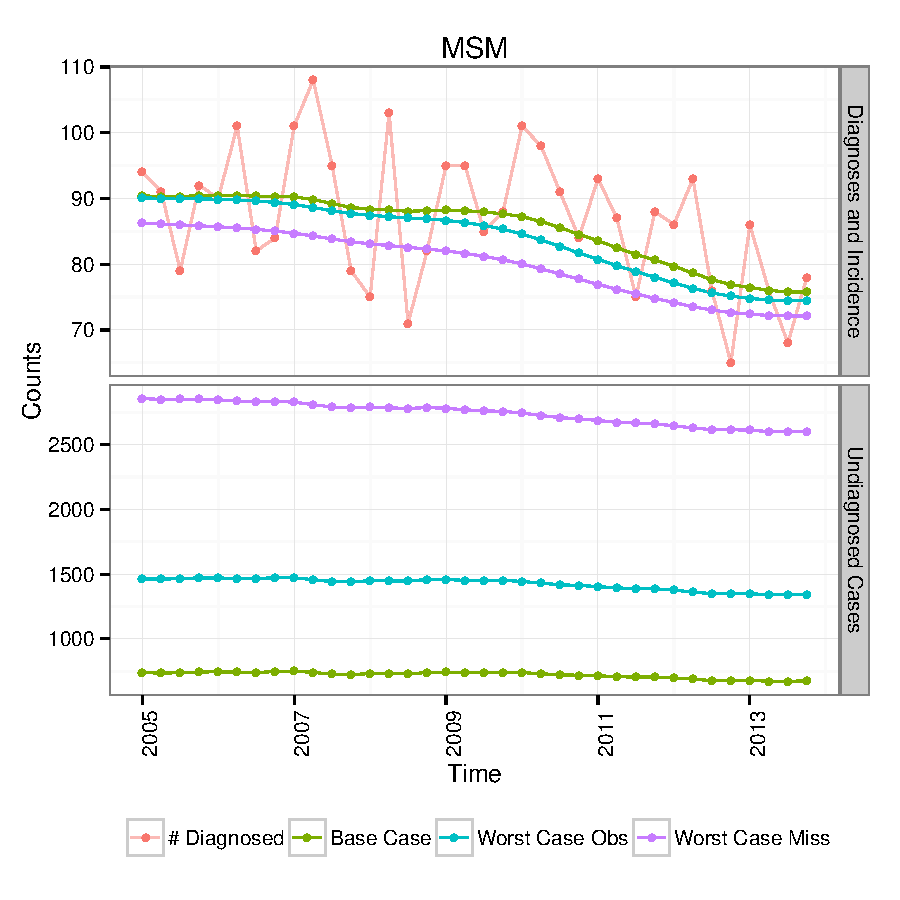
\includegraphics[width=\maxwidth]{figure/minimal-plot_subgroup_MSM} 

}

\caption[Observed diagnoses and estimated quarterly and undiagnosed counts over 2005-2013 in WA state, MSM]{Observed diagnoses and estimated quarterly and undiagnosed counts over 2005-2013 in WA state, MSM\label{fig:plot_subgroup_MSM}}
\end{figure}


\end{knitrout}


\begin{knitrout}\footnotesize
\definecolor{shadecolor}{rgb}{0.969, 0.969, 0.969}\color{fgcolor}\begin{figure}[]


{\centering 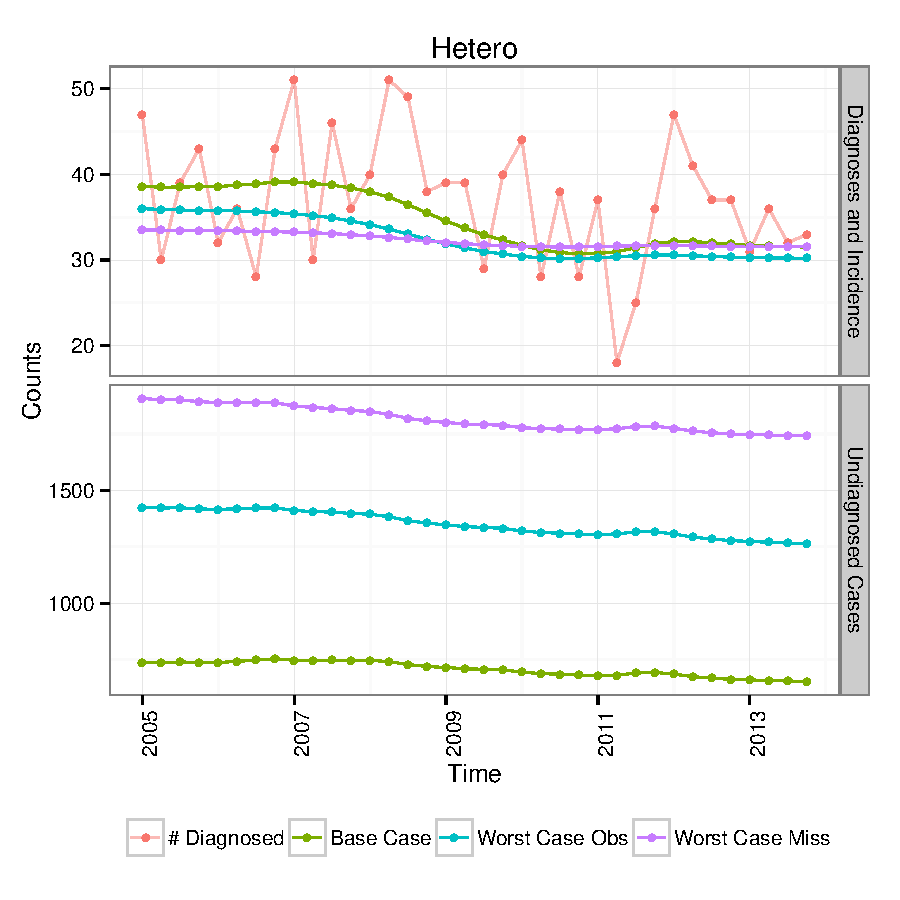
\includegraphics[width=\maxwidth]{figure/minimal-plot_subgroup_Hetero} 

}

\caption[Observed diagnoses and estimated quarterly and undiagnosed counts over 2005-2013 in WA state, Hetero]{Observed diagnoses and estimated quarterly and undiagnosed counts over 2005-2013 in WA state, Hetero\label{fig:plot_subgroup_Hetero}}
\end{figure}


\end{knitrout}


\begin{knitrout}\footnotesize
\definecolor{shadecolor}{rgb}{0.969, 0.969, 0.969}\color{fgcolor}\begin{figure}[]


{\centering 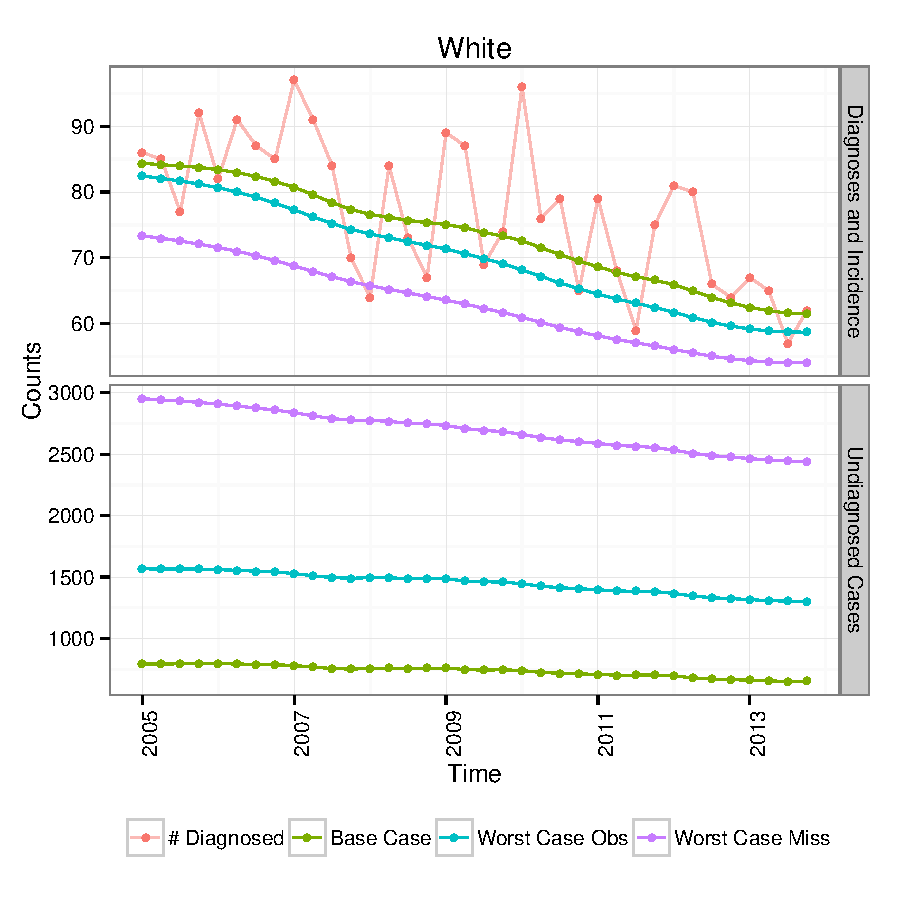
\includegraphics[width=\maxwidth]{figure/minimal-plot_subgroup_White} 

}

\caption[Observed diagnoses and estimated quarterly and undiagnosed counts over 2005-2013 in WA state, White]{Observed diagnoses and estimated quarterly and undiagnosed counts over 2005-2013 in WA state, White\label{fig:plot_subgroup_White}}
\end{figure}


\end{knitrout}


\begin{knitrout}\footnotesize
\definecolor{shadecolor}{rgb}{0.969, 0.969, 0.969}\color{fgcolor}\begin{figure}[]


{\centering 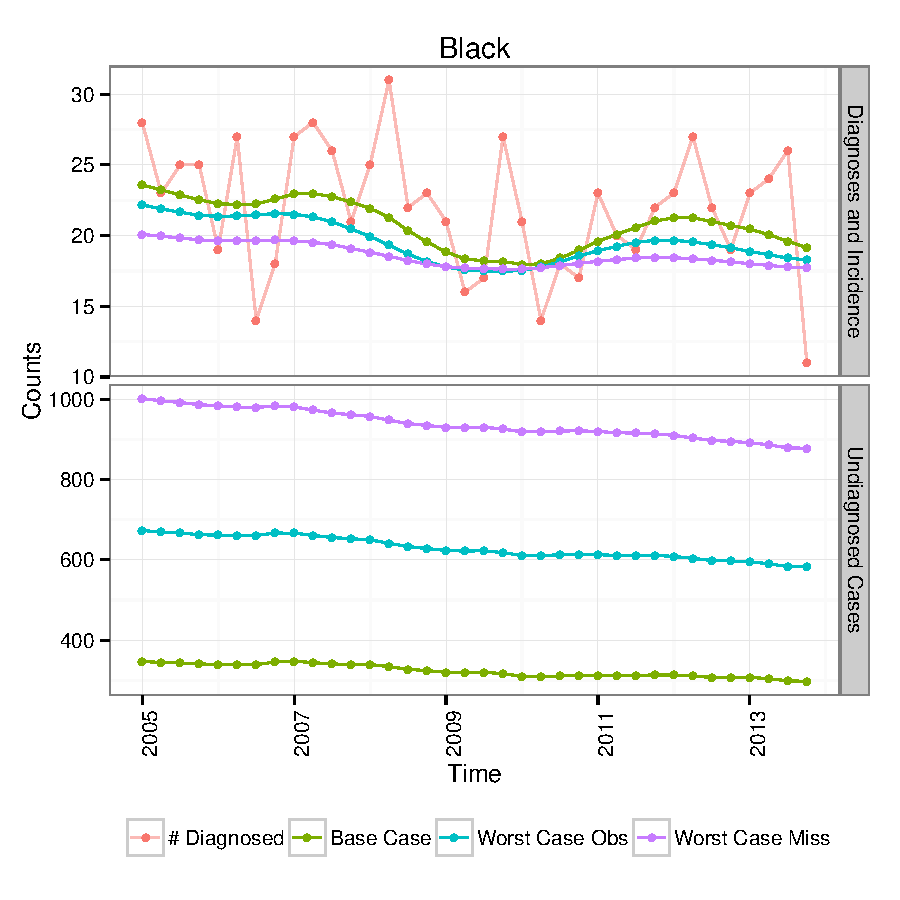
\includegraphics[width=\maxwidth]{figure/minimal-plot_subgroup_Black} 

}

\caption[Observed diagnoses and estimated quarterly and undiagnosed counts over 2005-2013 in WA state, Black]{Observed diagnoses and estimated quarterly and undiagnosed counts over 2005-2013 in WA state, Black\label{fig:plot_subgroup_Black}}
\end{figure}


\end{knitrout}


\begin{knitrout}\footnotesize
\definecolor{shadecolor}{rgb}{0.969, 0.969, 0.969}\color{fgcolor}\begin{figure}[]


{\centering 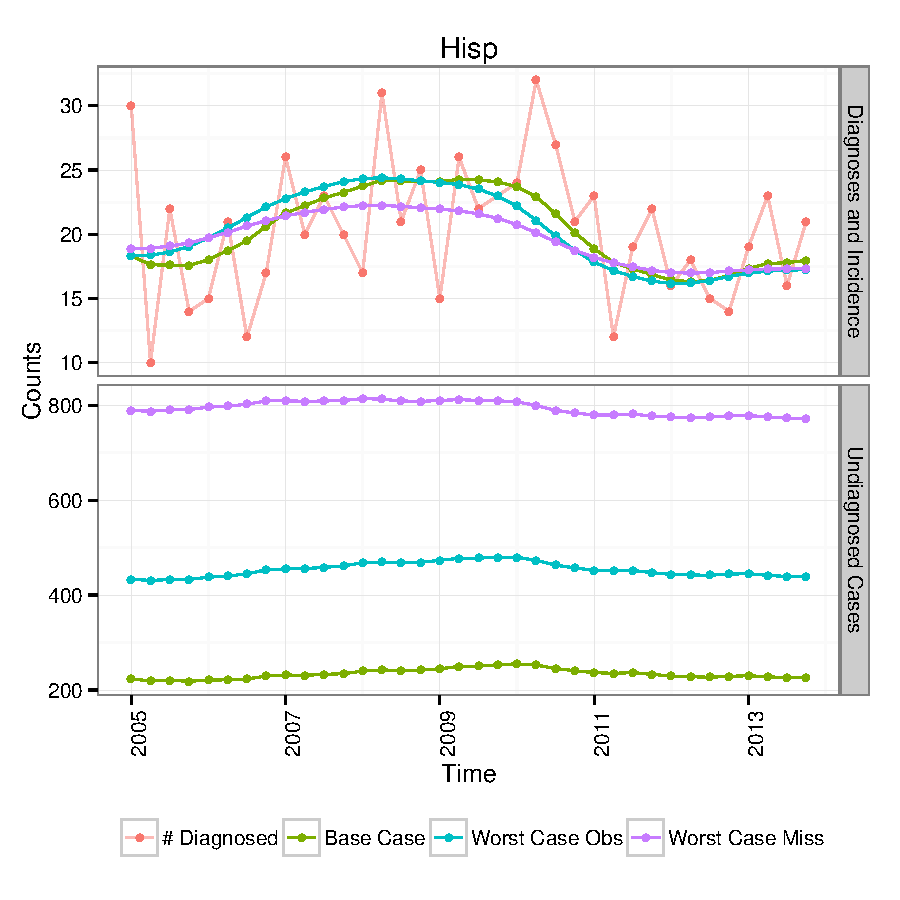
\includegraphics[width=\maxwidth]{figure/minimal-plot_subgroup_Hisp} 

}

\caption[Observed diagnoses and estimated quarterly and undiagnosed counts over 2005-2013 in WA state, Hisp]{Observed diagnoses and estimated quarterly and undiagnosed counts over 2005-2013 in WA state, Hisp\label{fig:plot_subgroup_Hisp}}
\end{figure}


\end{knitrout}


\begin{knitrout}\footnotesize
\definecolor{shadecolor}{rgb}{0.969, 0.969, 0.969}\color{fgcolor}\begin{figure}[]


{\centering 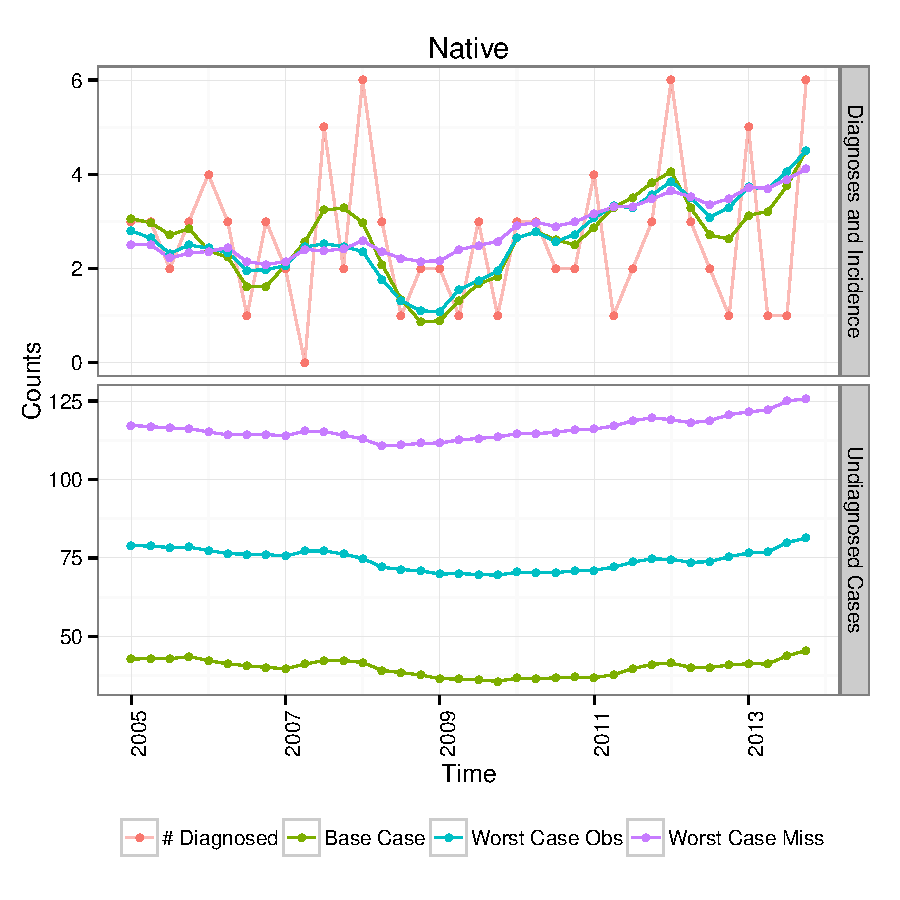
\includegraphics[width=\maxwidth]{figure/minimal-plot_subgroup_Native} 

}

\caption[Observed diagnoses and estimated quarterly and undiagnosed counts over 2005-2013 in WA state, Native]{Observed diagnoses and estimated quarterly and undiagnosed counts over 2005-2013 in WA state, Native\label{fig:plot_subgroup_Native}}
\end{figure}


\end{knitrout}


\begin{knitrout}\footnotesize
\definecolor{shadecolor}{rgb}{0.969, 0.969, 0.969}\color{fgcolor}\begin{figure}[]


{\centering 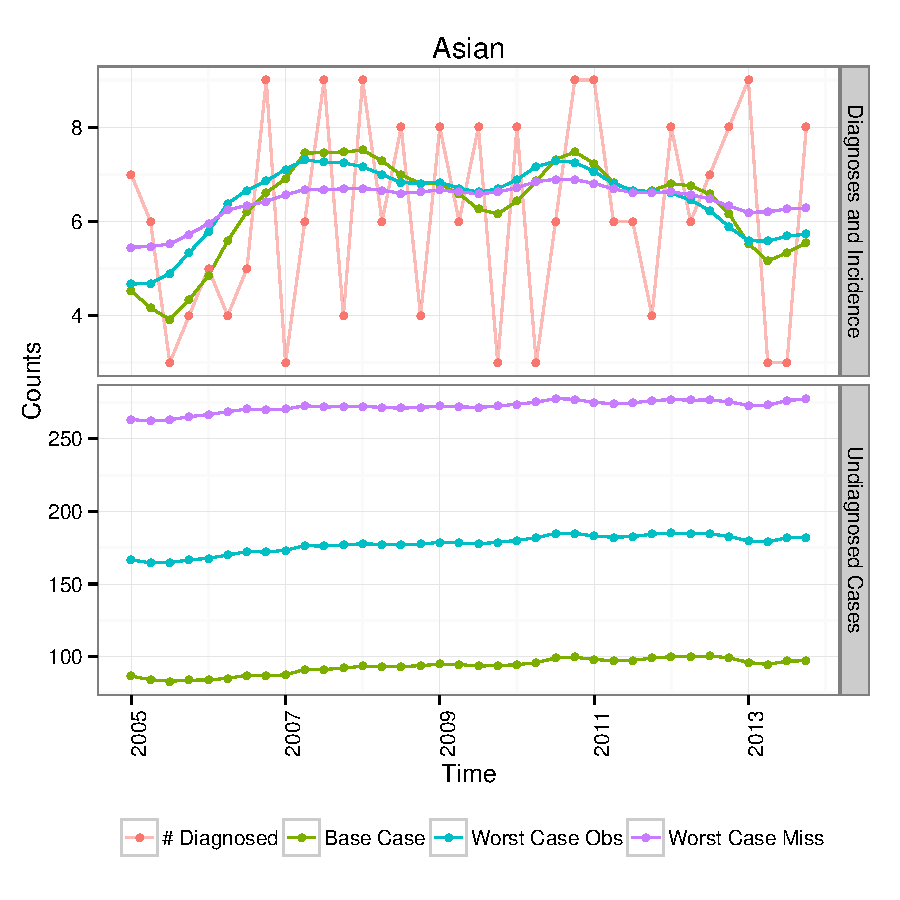
\includegraphics[width=\maxwidth]{figure/minimal-plot_subgroup_Asian} 

}

\caption[Observed diagnoses and estimated quarterly and undiagnosed counts over 2005-2013 in WA state, Asian]{Observed diagnoses and estimated quarterly and undiagnosed counts over 2005-2013 in WA state, Asian\label{fig:plot_subgroup_Asian}}
\end{figure}


\end{knitrout}


\begin{knitrout}\footnotesize
\definecolor{shadecolor}{rgb}{0.969, 0.969, 0.969}\color{fgcolor}\begin{figure}[]


{\centering 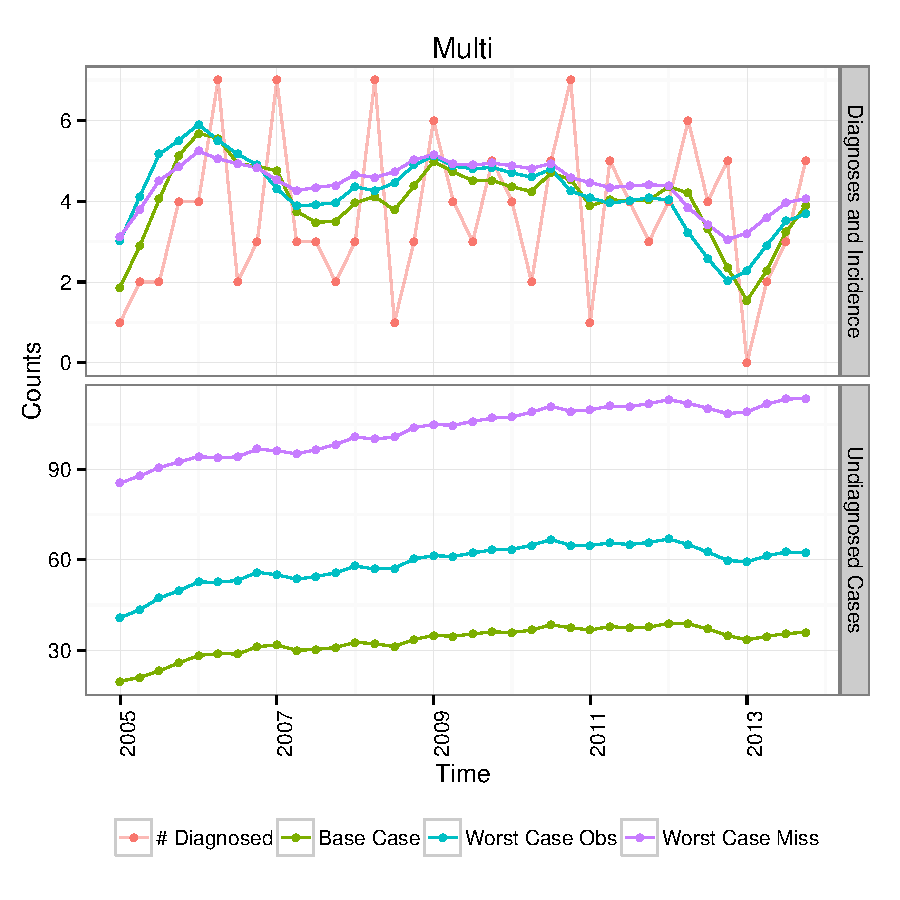
\includegraphics[width=\maxwidth]{figure/minimal-plot_subgroup_Multi} 

}

\caption[Observed diagnoses and estimated quarterly and undiagnosed counts over 2005-2013 in WA state, Multi]{Observed diagnoses and estimated quarterly and undiagnosed counts over 2005-2013 in WA state, Multi\label{fig:plot_subgroup_Multi}}
\end{figure}


\end{knitrout}


\end{document}


